The Probabilistic Event-based Risk calculator \citep{SilvaEtAl2014a} of the OpenQuake-engine is capable of calculating event loss tables, which contain a list of earthquake ruptures and associated losses. These losses my refer to specific assets, or the sum of the losses from the entire building portfolio (aggregated loss curves).
Using this module, it is possible to derive probable maximum loss (PML) curves (i.e. relation between a set of loss levels and corresponding return peridos of exceedance), as illustrated in Figure \ref{fig:pml}.

\begin{figure}[htb]
  \centering
      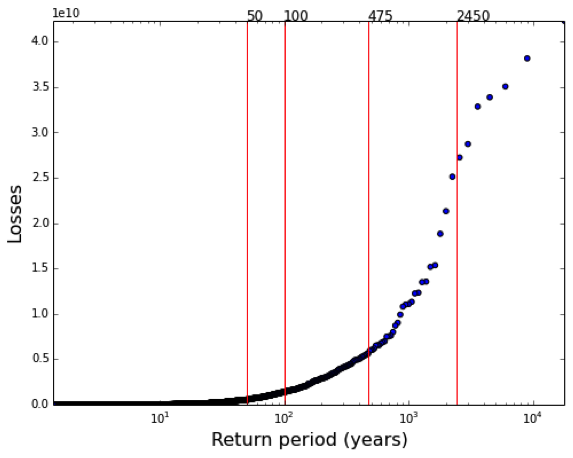
\includegraphics[width=8cm]{figures/pml_example.png}
  \caption{Probable Maximum Loss (PML) curve.}
  \label{fig:pml}
\end{figure}

To use this feature, it is necessary to use the parameter \verb=event_loss_table_folder= to specify the location of the folder that contains the set of event loss tables and stochastic event sets. Then, it is also necessary to provide the total economic value of the building portfolio (using the variable \verb=total_cost=) and the list of return periods of interest (using the variable \verb=return_periods=). This module also offers the possibility of saving all of the information in \verb=csv= files, which can be used in other software (e.g. Microsoft Excel) for other purposes. To do so, the parameters \verb=save_elt_csv= and \verb=save_ses_csv= should be set to \verb=True=.